%
% This is Chapter 1 file (chap1.tex)
%
\chapter{Introduction}\label{chap:chap1}

    \section{Prologue to Plasma}\label{sec:plas0}

        Our daily life is dominated by our interactions with the three classical states of matter:
        solid, liquid and gas. Plasma is the fourth state of matter and by far the most abundant
        one. In fact the observable universe is almost entirely made up of plasma (99.9\% of the
        universe) \citep{Boulos1994}. From the HII region around a huge star to the surface of a
        star, from the super hot Inter Galactic Medium to the inside of a plasma TV, plasma is
        everywhere. Given its abundance and ubiquitous nature, it becomes vitally important to study
        and understand plasma. In the rest of this chapter we define what constitutes a plasma
        (\Cref{sec:plas1}) and  discuss some of its salient properties and the laws of physics that
        govern it. We also shed some light on the local regions around Earth that are made up of
        plasma (\Cref{sec:plas2}) and discuss studying them (\Cref{sec:plas3}). We conclude the
        chapter with with a brief discussion of topics covered in this thesis. (\Cref{sec:plas4}).

    \section{Introduction To Plasma} \label{sec:plas1}

        The term ``plasma" comes from the ancient Greek word ``$\pi \lambda \acute{\alpha} \sigma
        \mu \alpha$" that means something that is moldable. It was first used in the modern context
        by \citet{Langmuir1928} to describe the ``region (around electrodes) containing balanced
        charges of ion and electrons".
        
        A plasma is a sub-type of ionized gas; a gas where significant fraction of the atoms have
        been ionized. There are specific criteria that distinguishes plasmas from other ionized
        gases (discussed later in this section), but first we consider the equations that govern the
        dynamics of charged particles (electrons and ions).

        As is with everything that has mass in the universe, a plasma's dynamics is governed by
        Newton's equation of motion:
        \begin{align}
            %\begin{split}
            \mathbf{F}_{\rm net} = \frac{d \mathbf{P}}{d t} & = m \frac{d^2 \mathbf{x}}{d t^2} \protect\footnotemark \label{eq:nwtn1}
        \end{align}
        \footnotetext{$\mathbf{F}_{\rm net} = m \frac{d^2 \mathbf{x}}{d t^2}$ is only valid when the
        particle is moving at speed much smaller than the speed of light.} where $\mathbf{F}_{\rm
        net}$ is the net external force acting on the system and \textbf{P} is its momentum. t is
        time, \textbf{x} is the position vector and $\frac{d}{dt}$ is the derivative with respect to
        time.
        
        For a charged particle with charge \textit{q}, moving with velocity \textbf{v} in an
        electromagnetic field with electric and magnetic field as \textbf{E} and \textbf{B}
        respectively, the electromagnetic force or Lorentz force is given as:
        \begin{align}
            \mathbf{F}_{\rm EM} = q \left( \mathbf{E} + \mathbf{v} \times \mathbf{B} \right)
            \label{eq:lorentz}
        \end{align}
        These equations (\Crefrange{eq:nwtn1}{eq:lorentz}) coupled with the four Maxwell's equations
        (\Crefrange{eq:maxwell1}{eq:maxwell4}) define the complete dynamics of a plasma.
        \begin{align}
            \nabla \cdot \mathbf{E} & = \frac{\rho}{\epsilon_\circ} \label{eq:maxwell1}\\
            \nabla \cdot \mathbf{B} & = 0 \label{eq:maxwell2}\\
            \nabla \times \mathbf{E} & = -\frac{\partial \mathbf{B}}{\partial t} \label{eq:maxwell3}\\
            \nabla \times \mathbf{B} & = \mu_\circ \mathbf{J} + \frac{1}{c^2} \frac{\partial \mathbf{E}}{\partial t} \label{eq:maxwell4}
            %\end{split}
        \end{align}
        where, $\rho$ is the charge density, $\epsilon_\circ$ is the permittivity of free space,
        $\frac{\partial}{\partial t}$ is the partial derivative with respect to time, $\mathbf{J}$
        is the current density, and c is the speed of light in vacuum.

        The most accurate way to study the behaviour of plasma is to track each particle
        individually using \Crefrange{eq:nwtn1}{eq:maxwell4}, all while accounting for all the
        fields, external as well as those arising because of the charge and motion of particles
        themselves. However, that method is almost impossible to implement not only because of
        difficulty in computing the field arising because of mutual interactions but also because of
        the huge number of particles involved. Consequently, scientists often fall back to
        statistical methods in their studies, such as applying kinetic equations that use physics
        based on ensemble averages (see \Cref{chap:chap2}) or by approximating the plasma as a fluid
        as is done in Magneto-hydrodynamics (MHD).

        Since even the lightest ion, a proton, is nearly 2000 times more massive than an electron
        and the dynamics of particles are often governed by their masses, both the time and length
        scales at which dynamics occur in plasmas are extremely diverse, even when one is studying
        the same phenomena for ions and electrons. Values of some of the parameters associated with
        plasma (generally referred to as \textit{plasma parameters}) can help in understanding the
        scales one is dealing with. Also, as will become apparent in \Cref{chap:chap2,chap:chap3},
        one may choose to focus on a specific scale depending on the interest or scope of the study.
        Here, we list some of the most relevant plasma parameters, what each one of them mean, and
        their mathematical expressions.\\
        \\
        \textbf{Debye Length} ($\lambda_{\rm D}$): The Debye length \index{Debye length} is the scale above which a
        plasma (with no net charge) maintains near charge neutrality --- $\rho \approx 0$ when
        $\rho$ is smoothed over a scale $\gtrsim \lambda_{\rm D}$. On scales smaller than
        $\lambda_{\rm D}$, particles behave as if it were interacting with other moving charges
        individually instead of a smooth macroscopic electromagnetic field. If we have sufficiently
        large number of particles inside a spherical volume with $\lambda_{\rm D}$ as the radius
        ($n_{\rm p} \lambda_{\rm D}^3 > 1$), then particles are shielded by its neighbours from the
        surrounding plasma (called \textit{Debye shielding}). On scales $\lesssim \lambda_{\rm D}$,
        random thermal motions of the particles give rise to isolated regions of non-zero charge
        density.  We would then expect $\lambda_{\rm D}$ to increase with plasma temperature.
        Indeed, for a plasma consisting of ionized hydrogen for which the protons and electrons have
        comparable temperatures, we define Debye length as:
        \begin{align}
            \lambda_{\rm D} & = \frac{\epsilon_\circ k_{\rm B} T_{\rm p}}{n_{\rm e} e^2}^{1/2} \label{eq:debye}
        \end{align}
        where $k_{\rm B}$ is the Boltzmann constant, $n_{\rm e}$ is the electron number density and
        $T_{\rm p}$ is the proton temperature. In order for a system to be classified as plasma, we
        must have the physical length scale (L) of the system much larger than its Debye length.
        \begin{align}
            \lambda_{\rm D} \ll L \label{eq:lambda}
        \end{align}
        \\
        \textbf{Ion-inertial Length \index{Ion-inertial Length}($d_{\rm j}$):} This is the length scale in plasma at which the
        electrons are decoupled from ions and the magnetic field is frozen in with the electrons.
        For species `$j$' of plasma (where $j = p^{+}$ for protons and $j = i^{n+}$ for any other
        ion with n positive charge)\footnote{In this thesis unless otherwise specified ion will
        refer to protons and two terms will be used interchangeably}, it can be written in terms of
        ion plasma frequency ($\omega_{\rm pj}$) as:
        \begin{align}
            d_{\rm j} = \frac{c}{\omega_{\rm pj}} \label{eq:ionint}
        \end{align}
        \\
        \textbf{Plasma Frequency \index{Frequency!plasma} ($\omega_{\rm pj}$)}\footnote{Note that `p' in $\omega_{\rm pj}$
        refers to plasma and not proton.}: It is the frequency at which any given species in plasma
        oscillates and is given by:
        \begin{align}
            \omega_{\rm pj} & = \left(\frac{n_{\rm j} q_{\rm j}^2}{\epsilon_\circ m_{\rm j}}\right)^{\frac{1}{2}} \label{eq:plasf}
        \end{align}
        \\
        \textbf{Cyclotron Frequency \index{Frequency!cyclotron} ($\Omega_{\rm cj}$):} In a magnetized plasma (a plasma which has
        a background magnetic field), due to the perpendicular direction of the magnetic force with
        respect to the particle's velocity, any non-stationary charged particle in a magnetic field
        gyrates around a point called the center of gyration. The frequency of gyration or cyclotron
        frequency is given by:
        \begin{align}
            \Omega_{\rm cj} & = \frac{q_{\rm j} B}{m_{\rm j}} \label{eq:cyclf}
        \end{align}
        where \textbf{B} is the background magnetic field. \\
        \\
        \textbf{Gyroradius \index{Gyroradius}}\textbf{($\rho_{\rm j}$)}: This is the radius of the circular path that a particle takes in
        the presence of a magnetic field, and is dependent on the ratio of thermal speed to that of
        cyclotron frequency.
        \begin{align}
            \rho_{\rm j} = \frac{w_{\rm j}}{\Omega_{\rm cj}} \label{eq:rho}
        \end{align}
        where $w_{\rm j}$ is the thermal speed of the particle. \\
        \\
        \textbf{Alfv\'en Speed \index{Alfv\'en Speed} ($V_{\rm Aj}$)}: It is the speed at which magnetic signals, like a
        fluctuation in the field, travel in a plasma. It depends on the strength of the magnetic
        field in the plasma as well the density and mass of the species and has the following
        expression:
        \begin{align}
            v_{\rm Aj} = \frac{B}{\sqrt{\mu_\circ \sum_{\rm j} n_{\rm j} m_{\rm j}}} \label{eq:alfv}
        \end{align}

    \section{Plasma in Near-Earth Environment} \label{sec:plas2}

        The Sun is the largest source of plasma in our solar system. Huge amounts of charged
        particles emanate from the Sun originating in its outermost atmospheric layer, called the
        Corona \citep{Parker1958,Parker1960,Parker1963,Gringauz1960,Neugebauer1962}. This constant
        outflow of particles is commonly called solar wind. The solar wind is often highly
        magnetized, is weakly collisional, travels at supersonic speed and is primarily composed of
        ionized hydrogen (i.e., protons) \citep{Marsch1982}. \Cref{tab:plaspar1} lists out some of
        the plasma parameters and their typical values for the solar wind at 1\,au.
        \Cref{fig:plas_para_wnd} shows the distribution of some of the parameters listed in
        \Cref{tab:plaspar1}.
        \begin{figure}
            \begin{center}
                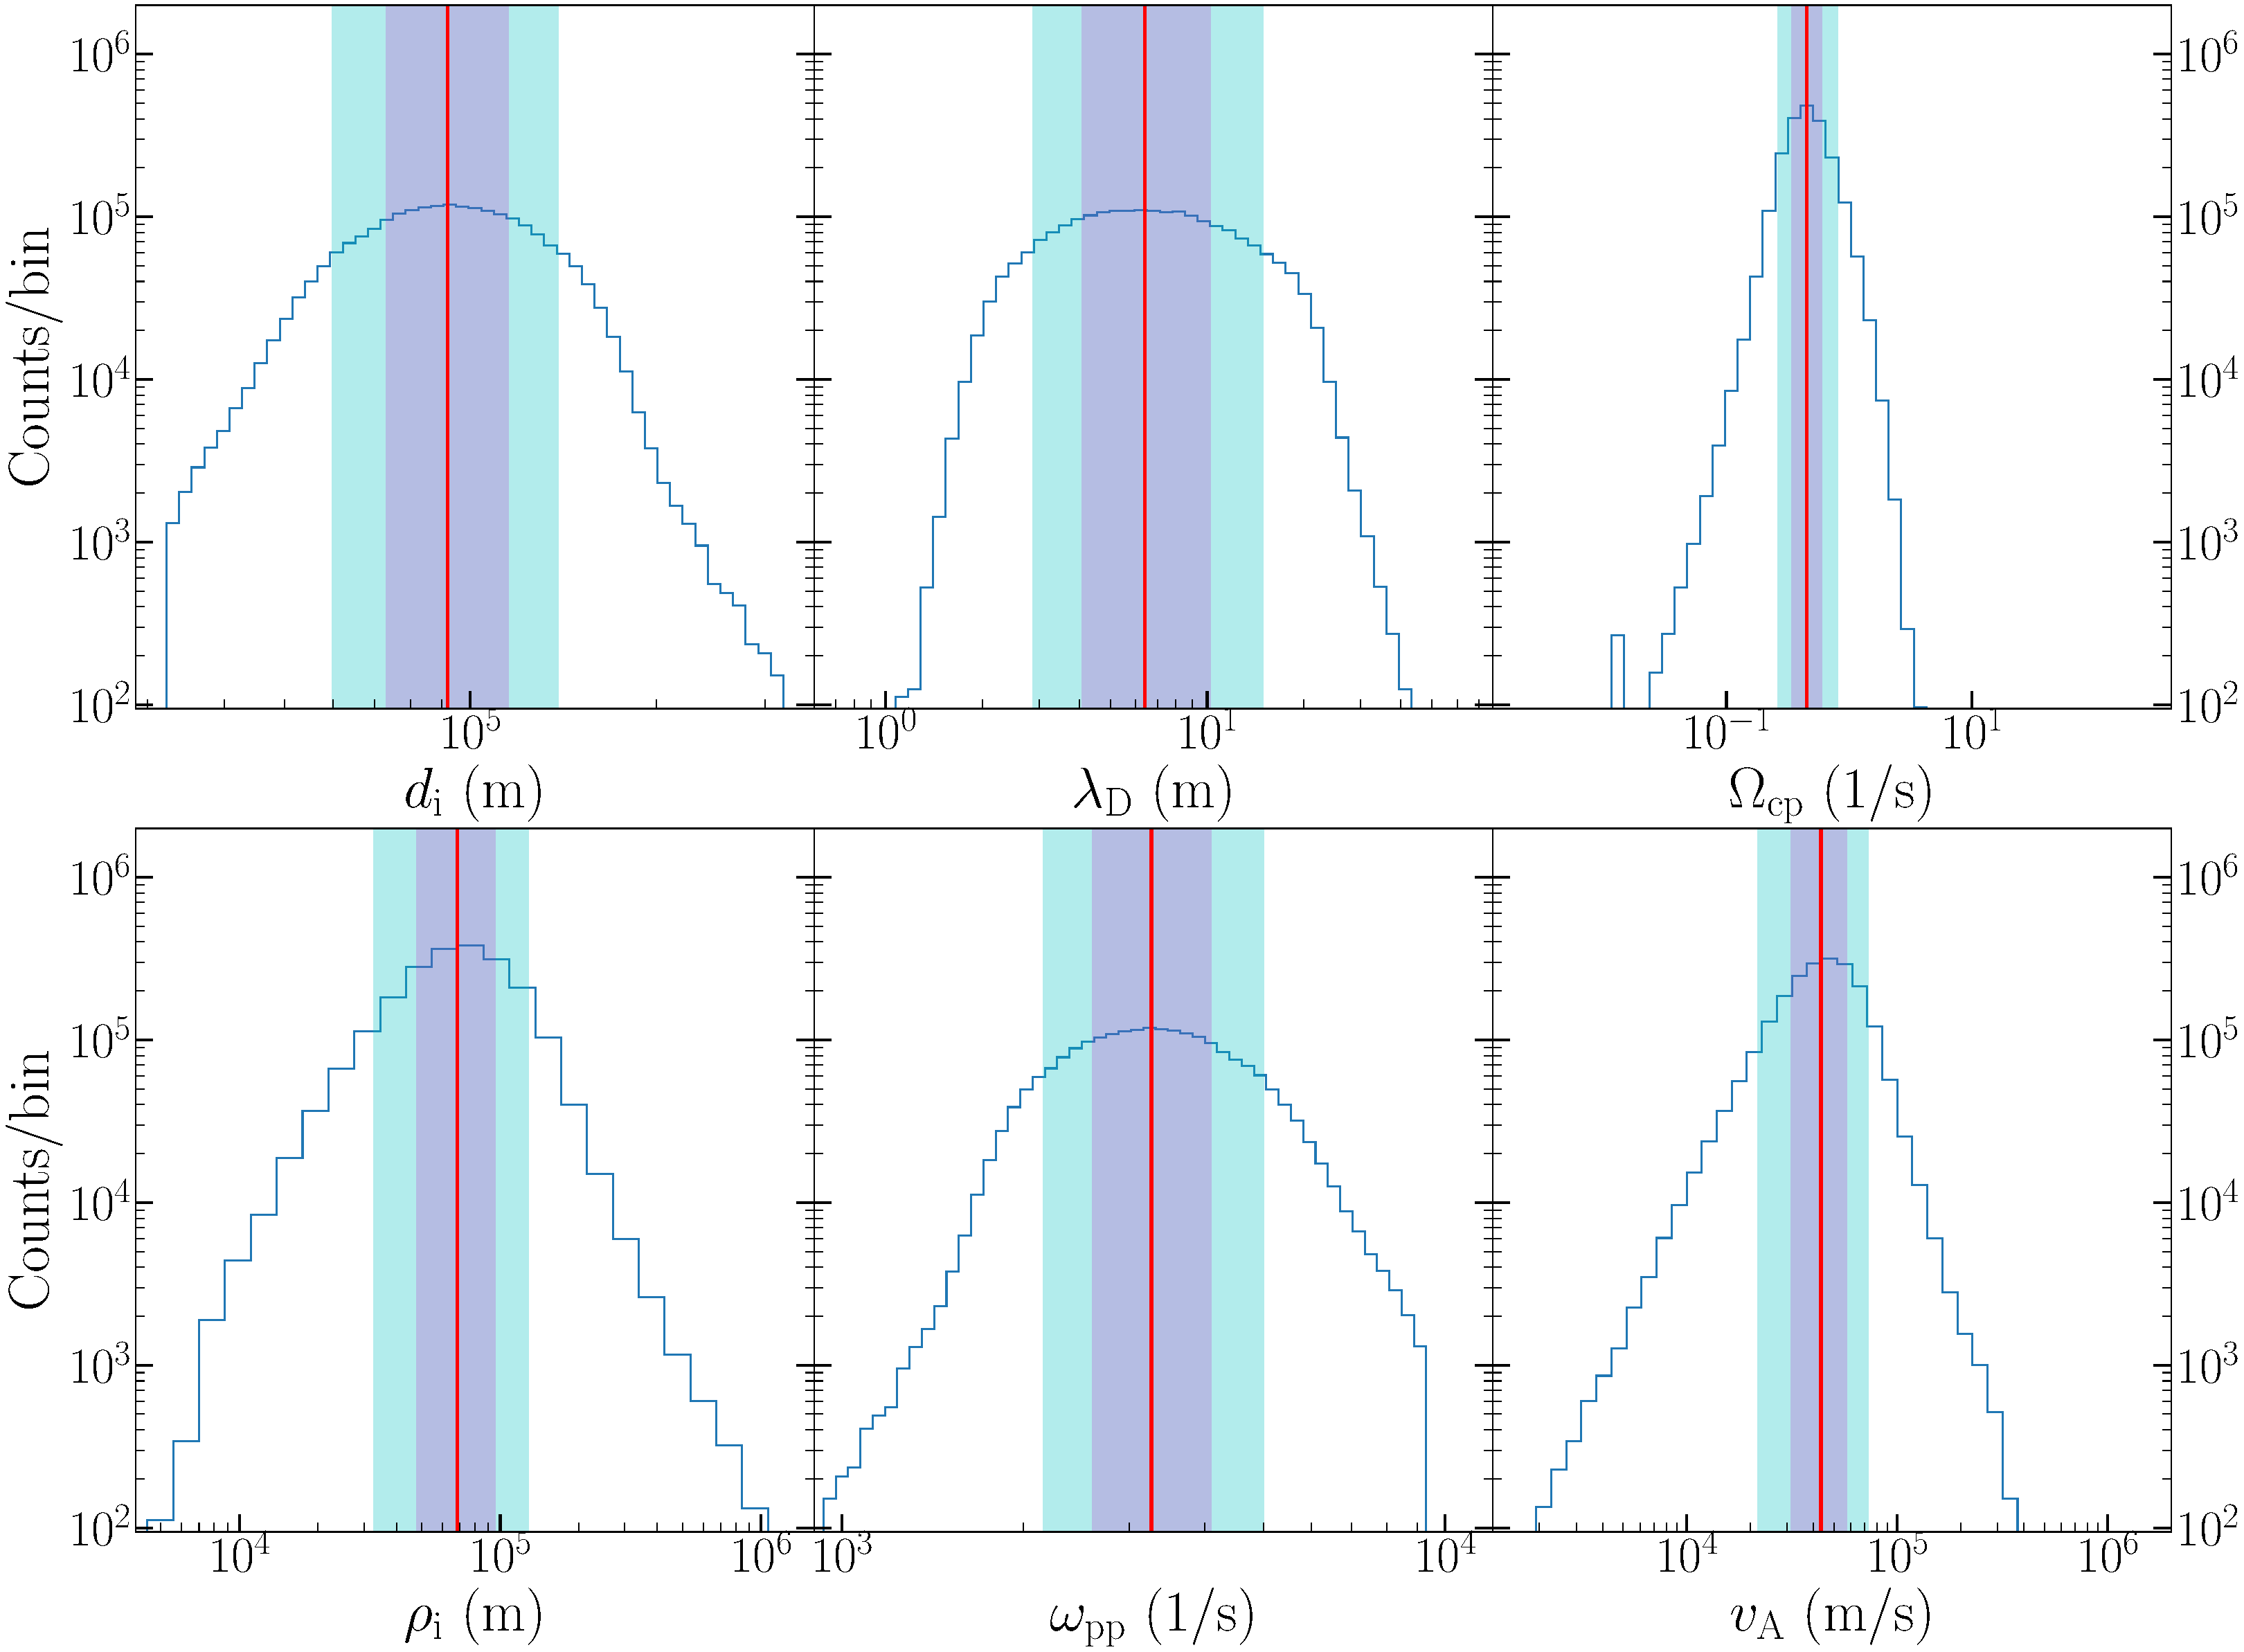
\includegraphics[width=1\textwidth]{figures/chap1/plasma_parameters_wnd.pdf}
                \caption[Plasma parameter distributions at 1\,au ]{Distribution of various plasma
                parameters near Earth, based on data from Wind spacecraft. Top row shows
                distribution for (from left to right) proton-inertial length ($d_{\rm i}$), Debye
                length ($\lambda_{\rm D}$), proton-gyrofrequency ($\Omega_{\rm cp}$) and the lower
                row shows (from left to right) proton-gyroradius ($\rho_{\rm i}$), proton-plasma
                frequency ($\omega_{\rm pp}$) and alfv\'en speed ($v_{\rm A}$). Red line shows the
                median value of each parameter, whereas the shaded region shows $10^{\rm th}$ to
                $90^{\rm th}$ (cyan) and $25^{\rm th}$ to $75^{\rm th}$ percentile (magenta) of each
                parameter.\protect\footnotemark}
                \label{fig:plas_para_wnd}
            \end{center}
        \end{figure}
        \footnotetext{\Cref{fig:plas_para_wnd} is based on data from Wind Spacecraft. See
        \Cref{sec:wind} for more details on data and spacecraft.}

        The Earth's local magnetic field, which arises as a result of dynamo action of its molten
        core \citep{Elsasser1956}, extends far into space (roughly 10 earth radii in the direction
        of the sun and $\sim$ 300 earth radii in the anti-sunward direction) and interacts with the
        incoming solar wind. This interaction gives rise to a plethora of structures.
        \Cref{fig:ms_earth} shows an artistic rendition of Earth's magnetosphere. The layer along
        which solar wind transitions from supersonic to subsonic speed is called the bow shock
        (region 1). The region immediately after the bow shock is called the magnetosheath (region
        2) and is comprised mostly of shock treated solar wind. This region is of special importance
        to the present work (see \Cref{chap:chap5,chap:chap7}). The region beyond the magnetosheath,
        towards Earth, where the pressure exerted by the solar wind and Earth's magnetic field are
        in equilibrium is called the magnetopause (region 3) and forms the boundary between Earth's
        magnetosphere (volume  around  Earth  where the influence  of  its magnetic field is felt
        (region 4)) and the solar wind. There is also a long magnetotail further away from the Sun,
        which extends far beyond the surface of the Earth (regions 5 and 6). The region closest to
        the surface (region 7) is called the plasmasphere, which is made up of relatively cooler
        plasma and is located above the ionosphere. The shape and size of all these structures vary
        greatly depending on the velocity and density of the incoming plasma, the strength of
        magnetic field, and solar activity.

        %Another distinct region of plasma close to the Earth is the ionosphere. It is part of the
        %upper region of Earth's atmosphere and forms because of photoionization of atoms by
        %ultraviolet radiation from Sun \cite[\S 4.4.3]{Wallace2006}. These radiation get absorbed
        %by around 90\,km above the surface and have enough energy and intensity to ``give rise to
        %sufficient number of free electrons" which helps in propagation of radio waves \cite[\S
        %4.4.3]{Wallace2006}. The structure of ionosphere is quite complicated and has a lot of
        %variability, both diurnal and seasonal. Owing to its complicated structure and dynamics it
        %is its own huge field of research and holds considerable interest for both geophysicists
        %and climatologists.\\

        \begin{table}[ht]
            \centering
            \caption[Plasma Parameters - Median values]{Plasma parameters and their typical values for different space plasmas.\protect\footnotemark}
            \begin{tabular}{ p{0.15\linewidth}  p{0.25\linewidth}  p{0.25\linewidth}
            p{0.25\linewidth}  }
                \hline
                \\
                Parameter & Solar Wind (0.15\,au ) & Solar Wind (1\,au ) & Magnetosheath \\ \\
                \hline
                \\
                $d_{\rm i}$ & 15,510 $\pm$ 6,200 m & 91,920 $\pm$ 42,000 m & 45,600 $\pm$ 9,900 m\\
                \\
                %\hline
                \\
                $\lambda_{\rm D}$ & 2.87 $\pm$ 1.98 m & 6.41 $\pm$ 6.20 m & 23.18 $\pm$ 8.00 m\\ \\
                %\hline
                \\
                $\Omega_{\rm cp}$ & 6.47 $\pm$ 2.70 1/s & 0.45 $\pm$ 0.26 1/s & 2.16 $\pm$ 1.00
                1/s\\ \\
                %\hline
                \\
                $\omega_{\rm pp}$ & 19,328 $\pm$ 7,300 1/s & 3,261 $\pm$ 1,500 1/s & 6,574 $\pm$
                1,500 1/s\\ \\
                %\hline
                \\
                $\rho_{\rm p}$ & 12,793 $\pm$ 8,500 m & 68,615 $\pm$ 48,000 m & 97,795 $\pm$ 69,000
                m\\ \\
                %\hline
                \\
                $V_{\rm A}$ & 102,503 $\pm$ 39,000 m/s & 43,390 $\pm$ 26,000 m/s & 94,256 $\pm$
                50,000 m/s\\ \\
                \hline
            \end{tabular}
            \label{tab:plaspar1}
        \end{table}
        \footnotetext{These values are based on datasets as described in \Cref{chap:chap4}.}

        \begin{figure}
            \begin{center}
                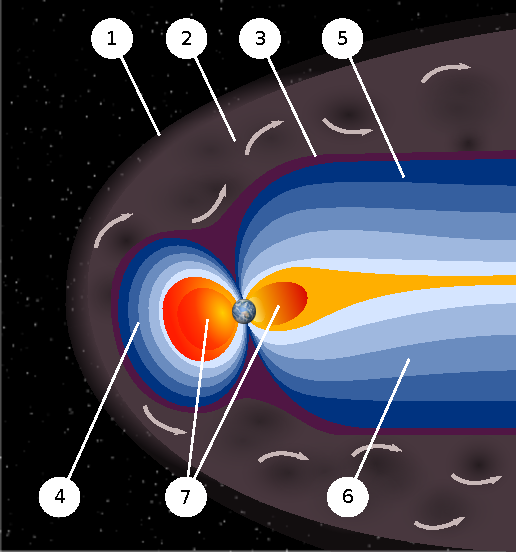
\includegraphics[width=1\textwidth]{figures/chap1/Magnetosphere_Levels.pdf}
                \caption[Earth's Magnetosphere's structure]{Artistic rendition of Earth's magnetosphere, its structure and different layers. The name of each numbered layer is 1.bow shock, 2. magnetosheath, 3. magnetopause, 4. magnetosphere, 5 and 6. tail lobes, 7. plasmasphere.\protect\footnotemark}
                \label{fig:ms_earth}
            \end{center}
        \end{figure}
        \footnotetext{Picture credit: https://commons.wikimedia.org/wiki/File:Magnetosphere\_Levels.svg}

    \section{Studying Space Plasmas} \label{sec:plas3}

        In the previous section (\Cref{sec:plas2}) we discussed two different kinds of naturally
        occurring plasma regions close to Earth. A complete theory of plasma would require us to
        understand the commonality as well as the uniqueness of each of these regions. Consequently,
        over the last century or so the scientific community has devised several methods to study
        them. From Guglielmo Marconi using an antenna on a kite to receive radio signals in 1901 to
        NASA launching a spacecraft costing more than a billion dollars (Parker Solar Probe (PSP))
        in 2018 to study the Sun from a closer distance than ever before, the community has been in
        a constant pursuit to understand them. 
        %\Cref{tab:spcmsn} lists out some of the major programs and missions along with mission
        %objectives, dedicated to such studies.\\
        %\begin{table}[ht] \centering \caption[Major space missions to study space plasmas]{Some of
        %    the major space missions to study space %plasmas \todo{update the table with full
        %    list}} \begin{tabular}{ | p{0.15\linewidth} | p{0.15\linewidth} | p{0.45\linewidth}|}
        %    \hline Spacecraft & Years Active & Major Objective \\
        %        \hline Voyager 1 \newline Voyager 2 & 1977 - \newline 1977 - & Study outer planets
        %         and interplanetary %medium \\
        %        \hline Wind & 1994 - & Study plasma processes in the solar wind near earth and in
        %        magnetosphere and %ionosphere\\
        %        \hline Helios A \newline Helios B & 1974 - 1982 \newline 1976 - 1985 & Observation
        %        of solar wind, electromagnetic fields, cosmic rays\\
        %        \hline MMS & 2016 - & Understanding magnetic reconnection and turbulence\\
        %        \hline Parker Solar Probe & 2018 - & Understanding Coronal heating\\
        %        \hline SoHo & 2018 - & Understanding Coronal heating\\
        %        \hline Ace & 2018 - & Understanding Coronal heating\\
        %        \hline STEREO & 2018 - & Understanding Coronal heating\\
        %        \hline \end{tabular} \label{tab:spcmsn} \end{table}

    \section{In This Thesis} \label{sec:plas4}

        Work done towards this thesis presents an incremental contribution towards understanding the
        nature and behaviour of space plasmas. \Cref{chap:chap2,chap:chap3} provide a theoretical
        background on plasma microkinetics and turbulence, respectively. \Cref{chap:chap4} gives a
        brief overview of all the datasets used in the present document and explains some of the
        data analysis techniques employed in \Crefrange{chap:chap5}{chap:chap7}.

        \Crefrange{chap:chap5}{chap:chap8} report the author's original work. \Cref{chap:chap5}
        discusses the intermittency in space plasmas and simulations as well as its co-development
        with linear instabilities. \Cref{chap:chap6} explores the heating of ions close to the Sun
        as a consequence of intermittent structures. \Cref{chap:chap7} discusses the competition
        between linear and non-linear processes using a statistical approach on six different
        datasets. \Cref{chap:chap8} presents an exploratory study of magnetic field reconstruction
        using machine learning (ML) techniques. \Cref{chap:chap9} provides a summary of the entire
        thesis and a guide for future work.